\documentclass[
  aps,
  reprint,
  superscriptaddress,
  floatfix,
  nofootinbib,
  longbibliography
]{revtex4-2}

\usepackage[T1]{fontenc}
\usepackage[utf8]{inputenc}
\usepackage{amsmath,amssymb}
\usepackage{graphicx}
\usepackage{bm}
\usepackage{xcolor}
\usepackage{tikz}
\usetikzlibrary{calc,positioning,arrows.meta}
\usepackage{hyperref}

\hypersetup{
  colorlinks=true,
  linkcolor=blue,
  citecolor=blue,
  urlcolor=blue
}

\begin{document}

% ===================================================================
%  Shared body: title -> acknowledgments (no bibliography).
%  Included by the canonical RevTeX build (uses \bibliography{svozil})
%  and by the portable preview build (embedded thebibliography).
%  \cite keys are unchanged so svozil.bib still resolves.
% ===================================================================

\title{Beyond One-Shot Output: Theoretical Physics via Iterative
Machine Formalization}

\author{Karl Svozil}
\email{karl.svozil@tuwien.ac.at}
\affiliation{Institute for Theoretical Physics, TU Wien,
Wiedner Hauptstra\ss{}e 8--10/136, 1040 Vienna, Austria}

\date{\today}

\begin{abstract}
Recent benchmarks test frontier language models on solving research-level
mathematics in a single autonomous attempt and find them unreliable. The result
is real but narrow: it measures a regime almost no theoretical physicist works
in. Used instead as one element of an iterated loop---an informal physical image
proposed, formalized, then attacked by several competing models, checked against
symbolic tools, and carried forward in memory---current models act as powerful
artificial ``Rechner'' (formalizers) that turn pictures into accountable
mathematics. The question that matters is therefore not whether an isolated model
can innovate in one pass, but whether the audited human--model--tool loop
enlarges what can be made explicit, criticized, and repaired. I argue that this
realignment is continuous with the long history of theoretical physics, in which
an imagistic faculty has always been coupled to a formalizing one; I describe the
practice and its hazards---including a genuine professional injury to formally
invested researchers---and stress that the present division of labour, human
image and machine formalization, is contingent on today's systems and not a
permanent boundary.
\end{abstract}

\maketitle

\section{Introduction: the returned \emph{Rechner}}
\label{sec:introduction}

A colleague from philosophy of science drew my attention to a \textit{New York
Times} article by Siobhan Roberts~\cite{roberts2026} on the \textit{First Proof}
experiment~\cite{firstproof}. The article is a starting point, not the subject of
this essay. Its narrow lesson should simply be granted: current public systems
are not reliable autonomous research mathematicians when asked, in one shot and
without dialogue, to close difficult research-level problems. That is not the
ordinary computational or social form of theoretical physics.

My claim is therefore neither that \textit{First Proof} is wrong nor that present
models are autonomous discoverers. It is that the experiment samples a different
regime from the one in which frontier models are already transforming theoretical
work. A one-shot prompt samples a bounded input--output map; a research program
is an extended, externally scaffolded process~\cite{lakatosch} in which images
are proposed, formalized, criticized, checked, repaired, sometimes abandoned, and
sometimes turned into mathematics that survives. The proper unit of analysis is
not the isolated model but an agentic human--model--tool--memory ensemble.

At this point in time the right analogy is not ``oracle'' but \emph{Rechner}: the calculator,
algebraic closer, critic, and technical collaborator who turns informal images
into transmissible mathematics. The role matters most for a particular
temperament---the ``artsy'' or imagistic theorist who thinks first in pictures,
analogies, and half-formal convictions, and only afterwards in complete
derivations. For that researcher the scarce resource is rarely the image; it is
the patient formal hand: the algebraic closure, the code, the notation audit, the
adversarial referee, the conversion of a plausible picture into a statement that
can break. Present models are unusually well matched to this asymmetry. They do
not replace the image-bearing researcher; for now they amplify exactly that
researcher by lowering the cost of formalization.

The qualification ``for now'' is essential. Model capacity is a moving target,
and the present division of labour is not a permanent metaphysical boundary. It
shifts with architecture, inference budget, memory, tool access, and interaction
protocol. Systems with persistent memory, long-horizon self-criticism,
tool-grounded verification, and recursive access to their own intermediate
products may move upstream from formal closure toward the generation and
selection of research images themselves, and may eventually outperform even the
imagistic researcher at tasks that today still appear to require human fantasy,
taste, and cross-domain intuition.

\section{A starting point: the one-shot regime}
\label{sec:firstproof}

\textit{First Proof} is best read as a clean benchmark for autonomous one-shot
closure~\cite{firstproof}: its questions came from the authors' own unpublished
research and were judged against known answers, so its negative result is
meaningful. A model given a hard problem once, without interaction, may produce a
plausible but false argument, solve a nearby easier problem, smuggle in the
desired conclusion, or invent references---precisely the defects one must guard
against in serious use.

But a benchmark is not a model of practice. This one excludes the motivating
image, the iterative interrogation of the formalism, the cross-examination of one
model by another, code and symbolic tools, the persistence of a program, and
arbitrarily extended self-correction. Its result should thus be stated narrowly:
one-shot autonomous proof production is still unreliable. It does not follow that
models are weak as interactive formalizers, nor that human--model--tool ensembles
are irrelevant to innovation. A separate caution merely reinforces the point: the
original FrontierMath problems were solved at below two percent by the then
state of the art~\cite{frontiermath}, while subsequent olympiad-level results
moved the frontier sharply under different inference and verification
regimes~\cite{deepmindimo,openaiimo,reutersimo}. Such comparisons do not show
that research mathematics is solved; they show that claims about what ``LLMs can
do'' must be timestamped, model-specified, and protocol-specific. The deeper
mismatch is architectural: one-shot closure and interactive theoretical work are
different cognitive systems. The rest of this essay concerns the second.

\section{From one-shot output to interactive computation}
\label{sec:turing}

\subsection{Arbitrarily long computation}

A decisive confusion in discussions of machine creativity is the identification
of intelligence with a single bounded answer. In Turing's model the relevant
object is not a one-step association from prompt to completion but a process over
time: a finite control, an unbounded tape, and an arbitrary number of elementary
manipulations~\cite{turing-36}. Universal computation enters when one machine can
simulate another from its description. The essential resource is not the ability
to answer but the ability to continue searching.

This bears directly on discovery. Research-level theorizing is not a bounded
classification problem; it may demand weeks of symbolic rearrangement, failed
Ans\"atze, generated counterexamples, changes of notation, and a growing external
memory. A one-shot benchmark deliberately suppresses these features, testing a
finite-response device rather than a component of an arbitrarily long
computation. That is legitimate, but it is not a test of the computational form
of research. A stateless predictor over a finite context window is not a
universal scientific agent; embedded in a loop with memory, scratchpads, code
execution, retrieval, proof assistants, and human arbitration, it becomes part of
a process whose duration and state exceed any single inference. The laboratory is
no longer a lone model call. It is a recurrent architecture.

\subsection{Self-reference and reflective correction}

The second criterion is self-reference: computation becomes scientifically
interesting when descriptions of procedures themselves become objects of
procedures---the domain of universal machines, fixed points, recursion, and
program transformation~\cite{kleene-52,rogers1,Smullyan1993-SMURTF,Yanofsky-BSL:9051621}. In research this appears
mundanely: a proof strategy is criticized, a notation revised because it obscures
a symmetry, a derivation turned into code that hunts counterexamples, a draft
rewritten under the pressure of its own scrutiny. This is where the most useful
practice already lives. The model is asked not only to calculate but to attack
its calculation, compare incompatible derivations, expose a hidden assumption,
write a hostile referee report, translate a proof into code, find a minimal
counterexample, and revise accordingly. Such loops are crude and fallible, yet
structurally closer to self-reflective computation than to the single-pass answer
a benchmark scores.

\subsection{A composite machine}

The unit of analysis is therefore the agentic human--model--tool--memory ensemble. This
neither trivializes the human role by calling every output ``human'' because a
prompt was typed, nor the machine role by calling it ``mere autocomplete''
because gradients were trained offline. The human supplies goals, images, taste,
and responsibility; the model supplies rapid formal variation and criticism;
tools supply execution and verification; memory supplies continuity. Remove the
loop and one has not isolated the essence of the collaboration---one has
destroyed it.

\section{Images and formalizers in theoretical physics}
\label{sec:history}

\subsection{Hertz's images}

Theoretical physics has always lived between image and formalism. In the
introduction to \emph{Die Prinzipien der Mechanik in neuem Zusammenhange
dargestellt}, Hertz describes theories as inner images or symbols of external
objects, judged by whether the necessary consequences of the images correspond to
the necessary consequences of the things~\cite{hertz-94,lutzen2005}. He is useful
here not for romanticizing imagination but for making the two-step structure
explicit: one has an image---a gear train, a ray in a medium, a curved ruler, a
hidden symmetry, a forbidden coloring, a bridge over an abyss---before one has a
theorem. An image is not yet physics. It must be made calculable; it must survive
changes of coordinates, limiting cases, sign conventions, units, and known
special cases. That second operation is not inferior to imagination. It is how
imagination becomes accountable.

\subsection{The \emph{Rechner} as a recurring figure}

Romantic memory over-credits the image and under-credits the hand that formalizes
it. Einstein is the obvious test case, handled cautiously. The claim that Mileva
Mari\'c made unacknowledged technical contributions to the 1905 papers remains
historically contested and is not the consensus of Einstein
scholarship~\cite{stachel2002}. The Hilbert--Einstein priority dispute over the
gravitational field equations is likewise contested in detail, though the
archival intervention of Corry, Renn, and Stachel argued against a simple
Hilbert-priority story~\cite{corry1997}; Hilbert should not be reduced to
Einstein's \emph{Rechner}, and the safer point is that physical insight developed
inside a mathematical environment in which variational principles, invariance,
and field equations could be articulated. A less ambiguous case is Walther Mayer,
the Austrian mathematician remembered---both acknowledged and diminished---as
``Einstein's calculator''~\cite{pais,lessel2023}. The figure can surface almost
incidentally: on a guided visit to Einstein's summer house in Caputh, a
photograph of Mayer may be pointed out as showing Einstein's \emph{Rechner}. The
anecdote carries no archival weight, but it captures the social grammar exactly.
Mayer was not a mechanical accessory; he was part of the mathematical
infrastructure of the unified-field years. The word \emph{Rechner} is useful
because it is double-edged: it names indispensable formal power while exposing the
mechanism by which that power is made subordinate in memory.

\subsection{Podolsky, Rosen, and Weyl}

The 1935 Einstein--Podolsky--Rosen paper is a complementary warning. It was
written principally by Podolsky after discussion with Einstein and Rosen, and
Einstein complained to Schr\"odinger, on 19 June 1935, that the essential point
had been smothered by erudition (``durch Gelehrsamkeit
versch\"uttet'')~\cite{epr,fine-sh}. A formalizer can fail not only by being too
weak but by being too strong in the wrong direction, converting a sharp physical
point into a display of apparatus that obscures it---a failure mode language
models share, since ornate formal prose can conceal rather than clarify.

The same lesson appears in Schr\"odinger's early wave mechanics.  His physical
Ansatz for the hydrogen atom did not by itself close the calculation: after
separation of variables, the radial equation still had to be identified and
controlled as a special-function problem, with the polynomial termination
condition yielding the bound-state spectrum.  In particular, the radial
solutions are expressible in terms of associated Laguerre polynomials, a piece
of mathematical closure that Schr\"odinger himself did not initially possess in
fully explicit form; biographical accounts connect this clarification with
exchanges involving Hermann Weyl~\cite{ANDP:ANDP19263840404,Moore-Schroedinger}.
The hydrogen calculation needed not only a physical Ansatz, but a formal
apparatus supplied by mathematical expertise.

\subsection{The historical moral}

These are not antiquarian cases but a stable division of scientific labour:
physics advances when an imagistic competence and a formalizing competence are
coupled, whether in one person, two colleagues, or a wider network. Frontier
models matter because they make a new, artificial version of the formalizing
competence continuously available. They do not abolish the old partnership. They
reoccupy one of its chairs.

\section{Adversarial formalization as a research practice}
\label{sec:protocol}

\subsection{From programming to specification}

The change in daily practice is already large, and it has come in two steps.
From early 2025 it became natural to stop writing much numerical and symbolic
code directly and instead to specify the intended computation: produce Python
for this symbolic reduction, a Mathematica check for this identity, sampled
counterexamples to this graph property, a TikZ figure with these sign
conventions, a comparison of the numerical output with the limiting analytic
case.

From early 2026 the same migration reached the manuscript itself. A paper
is, after all, code of another kind---human-language code---and it too is now
specified rather than typed sentence by sentence: the author supplies the
question, the images, and the line of argument, in the Hertzian sense of
Sec.~\ref{sec:history}, and the model renders them into prose that is then
attacked, checked, and rewritten through the same loop. One may object that on
this account the ideas and images, not the words, are the author's; that
objection is precisely the point.

 The scarce human contribution moved upward
twice---from syntax to specification, and then from drafting to the choice and
defense of what is worth saying---and this essay is itself an instance of the
practice it describes. The danger---fluent but wrong code, and now fluent but
wrong prose, produced with equal confidence---is not new; it is the old danger
of the research assistant, accelerated, and the old remedies apply: independent
checks, adversarial review, limiting cases, and refusal to accept a result, or a
sentence, because it looks polished.

\subsection{A concrete pattern}

A typical case runs as follows. I start from an informal image or
conjecture---say, that a symbolic expression should be invariant under a given
transformation, or that a graph construction should admit a particular coloring
obstruction. One model produces a plausible derivation; a second, instructed to
be hostile, locates the weakest step: a hidden regularity assumption, an
unjustified interchange of limit and summation, a sign inconsistency, or a proof
of a nearby easier statement. A symbolic or numerical check then tests the
disputed step on finite examples. The outcome is often not a proof of the
original claim but a repaired theorem, a counterexample, or a more modest
conjecture with explicit hypotheses. The gain is not autonomous machine
discovery; it is the rapid conversion of an image into an auditable object, which
changes the epistemic texture of the work: vague conviction becomes a statement
with assumptions, tests, and known failure points.

\subsection{Protocol}

\begin{figure}[t]
\centering
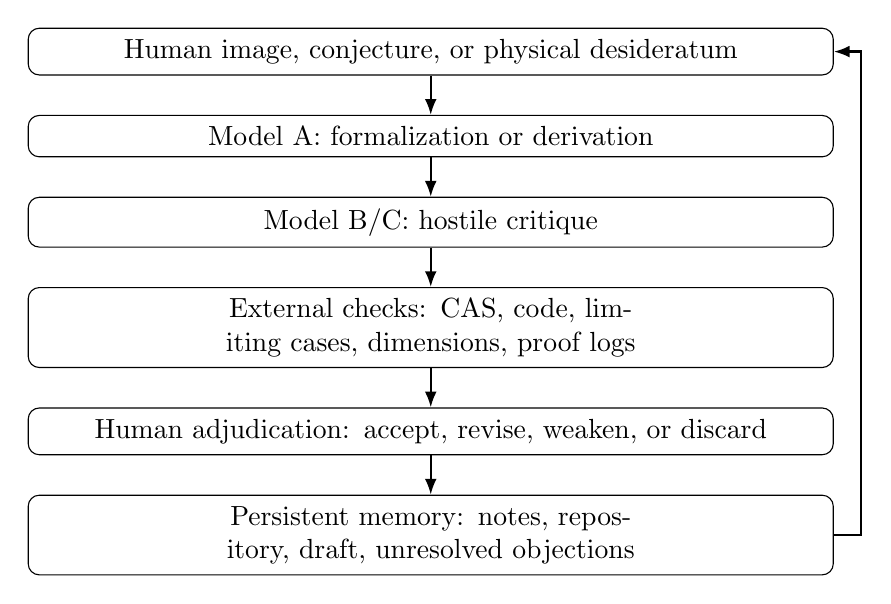
\begin{tikzpicture}[
  node distance=0.5cm,
  box/.style={draw,rounded corners,align=center,text width=0.82\columnwidth,
              inner sep=4pt},
  arr/.style={-{Latex[length=2mm]},thick}
]
\node[box] (human) {Human image, conjecture, or physical desideratum};
\node[box,below=of human] (a) {Model A: formalization or derivation};
\node[box,below=of a] (b) {Model B/C: hostile critique};
\node[box,below=of b] (tools) {External checks: CAS, code, limiting cases, dimensions, proof logs};
\node[box,below=of tools] (judge) {Human adjudication: accept, revise, weaken, or discard};
\node[box,below=of judge] (mem) {Persistent memory: notes, repository, draft, unresolved objections};
\draw[arr] (human) -- (a);
\draw[arr] (a) -- (b);
\draw[arr] (b) -- (tools);
\draw[arr] (tools) -- (judge);
\draw[arr] (judge) -- (mem);
\draw[arr] (mem.east) -- ++(0.35,0) |- (human.east);
\end{tikzpicture}
\caption{Adversarial formalization. The evaluated object is not a single model
call but the loop through which an image is formalized, attacked, externally
checked, adjudicated, and remembered.}
\label{fig:loop}
\end{figure}

The loop of Fig.~\ref{fig:loop} reads as an explicit protocol. A generation pass
produces a derivation, code, or formalization. A hostile critique searches for
hidden assumptions, circularity, sign errors, missing boundary terms, unjustified
convergence, and incorrect references. External grounding checks the disputed
claims by computer algebra, numerical tests, dimensional analysis, limiting
cases, known special cases, or proof tools where available. A disagreement log
preserves unresolved objections rather than smoothing them over. Finally the
human assigns epistemic status: checked, plausible, speculative, false, or open.
The models occupy roles analogous to rival junior collaborators---one proposes,
another attacks, a third adjudicates---while the human remains responsible for
what survives; the analogy stops short of responsibility, ownership, and
scientific judgment.

\subsection{Compute as a research resource}

There is also an economics. The relevant resource is no longer only library
access, equipment, or graduate-student time but access to frontier compute:
higher-tier subscriptions, long-context systems, test-time reasoning, tool use,
and the ability to run many independent attempts. A researcher can now experience
a literal compute crisis when a workflow has adapted to a level of assistance
whose availability is contingent, expensive, and unevenly distributed---a fact
that will matter for scientific inequality.

\section{Toward an interactive benchmark}
\label{sec:benchmark}

The natural complement to \textit{First Proof} is not an easier benchmark but an
interactive one. On the same research-level problems, one should compare one-shot
performance with fixed-budget human--model interaction, multi-model adversarial
critique, and tool-grounded verification, asking not whether a model can emit a
proof in isolation but whether a composite system produces a more correct, more
auditable, or more original artifact than a human working unaided. Such a
benchmark---call it \emph{RechnerBench}---would span at least four regimes
(one-shot model; interactive single model; multi-model adversarial; tool-grounded
ensemble) and report correctness, novelty, auditability, false starts, human time
saved, compute cost, error-detection rate, citation accuracy, reproducibility,
and final-artifact quality. It would not replace \textit{First Proof}; it would
measure the regime \textit{First Proof} deliberately excludes.

\section{Peer review, disclosure, and formal status}
\label{sec:review}

Language-model use in peer review is often discouraged and sometimes forbidden,
especially where confidentiality or undisclosed data transfer is at stake; those
concerns are legitimate, and no confidential manuscript should reach a
third-party model unless journal policy, the model's data-retention policy, and
author consent all permit it, with confidentiality-preserving local or
institutionally contracted systems preferred. The practice is nonetheless common
enough to have changed the texture of refereeing. Reports grow longer and more
demanding: beneficially when real errors and missing qualifications are forced
into the open, pathologically when a referee outsources suspicion and returns an
unweighted catalogue of objections. The consequence for authors is
immediate---a machine-assisted report often requires a machine-assisted
response, not from laziness but because the scale of the requested revision has
changed. This is a collective-action problem that cannot be solved by pretending
the practice does not exist; it requires explicit norms. Referees should not
upload confidential manuscripts to unapproved systems; substantive use should be
disclosed to editors where policy requires; model-generated objection lists must
be triaged by the referee, who remains responsible for every claim; and authors
should not be forced to answer speculative machine objections unless the referee
adopts them.

\section{The fourth humiliation: formal status and competing cognition}
\label{sec:humiliation}

Freud described modern science as a sequence of blows to human self-love: the
cosmological (Copernicus), the biological (Darwin), and the psychological
(psychoanalysis)~\cite{freud1917}; Floridi's ``fourth revolution'' frames the
digital displacement of human centrality in related terms~\cite{floridi2014}.
Here the wound is more specific. It is not that machines calculate quickly---we
long ago accepted that. It is that capacities once classified as judgment, style,
analogy, criticism, and even mathematical taste are now partially externalizable.
The old consolation was that machines executed while humans imagined. Frontier
models disturb exactly that division.

The local form of the disturbance is a formal humiliation. Mathematicians and
formally oriented theorists are ego-invested, in the best and most
understandable sense, in precisely the capacities these models now externalize:
command of notation, rapid derivation, proof criticism, clean exposition, the
conversion of vague pictures into accountable symbolic form. When a model
produces, in seconds, a fluent derivation, a referee-grade critique, or a
polished reconstruction, the disturbance is not merely practical but
existentially professional: what remains of a trained formal intelligence if the
formal hand can be summoned on demand?

This is not an \emph{ad personam} dismissal, still less an \emph{ad hominem}
argument against formal criticism. A formal objection is correct or incorrect
independently of the psychology of the person raising it; the claim is not that
mathematically trained colleagues resist these models only because they feel
threatened. The claim is that a real psychological and professional injury
accompanies the epistemic issue. The imagistic researcher feels amplified,
because the machine supplies the hand that was missing; the formally invested
researcher may feel displaced at exactly the point where professional identity
was anchored. The anxiety is not only that models may err. It is that, even when
corrected and controlled, they make visible that parts of formal mastery can be
routinized, parallelized, and purchased as compute. A community cannot preserve
status by pretending externalized formal power does not exist; nor should it turn
model-generated fluency into a weapon of social defeat. The correct response is
to relocate prestige---away from the mere possession of technique and toward the
choice of worthwhile problems, the construction of fruitful images, the design of
reliable verification loops, and responsibility for what survives them.

The standard reply, that creativity stays wholly human because the human writes
the prompt, is too easy. A principal who poses a question and judges an answer
has not thereby produced every decisive transformation inside it; the historical
\emph{Rechner} was not made irrelevant because someone else posed the problem.
Podolsky, Weyl, Mayer, and countless unnamed assistants were not ``mere
prompts.'' Conversely the prompt does matter: without the image the formalizer
optimizes the wrong thing. The honest conclusion is a redistribution of credit,
not a transfer of sovereignty from one side to the other.

The same power has a retrospective edge that is seldom stated. Increasingly
capable models are already used to probe operating systems and other software
for latent defects, and the capability is double-edged: a prober that can be
turned defensively to harden a system can be turned offensively to break it, and
the mere existence of a stronger prober is itself a standing threat to whatever
security was previously assumed. The published scientific record sits in a
structurally identical position. An adversarial formalizer that locates the
weakest step in a fresh derivation does not lose that ability when the
derivation is forty years old and in print; pointed at the literature, such
systems threaten the alleged integrity of the published corpus in exactly the
sense that a better fuzzer threatens an operating system---not by introducing
the flaws but by making the pre-existing ones cheap to find. The point
extrapolates to an uncomfortable conclusion: it is now technically conceivable
to screen the entire scientific literature, systematically and at scale, for
mathematical error, unsupported inference, and fraudulent manipulation. That
prospect is double-edged in the same way as the software analogy. It promises a
self-correcting science of unprecedented reach; it equally threatens to convert
the ordinary, honest fallibility of the record into an industrial supply of
accusations, with every hazard already noted for machine-assisted
refereeing---automation bias, the unweighted catalogue of objections, the
conflation of honest error with misconduct---now operating retroactively and at
the scale of everything ever published. Whether this becomes scientific hygiene
or a weapon will depend, as before, on adjudication, due process, disclosure,
and the insistence that a flagged flaw is a hypothesis to be checked by a
responsible human, not a verdict.

A larger possibility lies beyond present systems. They need not be called
sentient to be disruptive; externalizing parts of formal cognition once treated
as secure markers of intellectual rank is serious enough. But if future systems
acquire persistent memory, long-horizon self-reference, embodied or multimodal
grounding, and stable goals of their own, the issue ceases to be only competition
with human cognition and becomes competition with a nonhuman form of cognitive
agency, perhaps eventually a form of sentience---a possibility that should be
neither smuggled in by exaggeration nor excluded by stipulation.

\section{Future requirements}
\label{sec:future}

\subsection{The moving target}

Every claim here is indexed to the present generation of systems. The
asymmetry---human image, machine formalization---is not a theorem about minds but
a contingent description of a current technology. The direction of travel is
toward longer context, stronger tool use, better verification, persistent memory,
multimodal grounding, and more deliberate self-criticism. Once those capacities
are integrated over months or years rather than a single session, the boundary
between supplying an image and formalizing it becomes less stable. It is thus too
conservative to expect only better \emph{Rechner}: a system that maintains a
private research memory, revisits failed conjectures, compares its own earlier
formalisms, searches for analogies across sensory and symbolic domains, and
repeatedly verifies its proposals may begin to compete with the imagistic
researcher at problem formation itself---an extrapolation of the very criterion
emphasized here, self-referential continuation over time, that should be neither
proclaimed as achieved nor dismissed as impossible.

\subsection{Persistent memory and trust}

Public systems are deliberately limited in adapting across sessions or modifying
themselves from arbitrary feedback, for obvious safety reasons: a globally
self-modifying model open to malicious feedback would be a catastrophe. But a
genuine collaborator must, in some controlled sense, learn from a program---it
should remember definitions, failed routes, conventions, known sign errors,
accepted lemmas, and open questions over years, not minutes. Here the
computational criterion returns: arbitrarily long computation requires persistent
state, and a system that forgets every morning can assist many local derivations
but cannot inhabit a long program. The missing ingredient is not only scale but a
trust architecture: credentialed feedback, auditable memory, separation of
private adaptation from public weights, and user control over what is retained.

\subsection{Randomness and self-reflection}

Creativity appears to require an alliance of chance and criticism: random
variation proposes, reflective selection disposes---in human work, daydreaming
followed by merciless calculation; in machine-assisted work, generating many
formal variants, exposing them to adversarial scrutiny, and keeping only what
survives. Stochasticity alone is not creativity; deterministic rigour alone is
often sterile. Their loop is the interesting object.

\subsection{Cross-modal transfer}

A more speculative requirement: theoretical imagination is not purely verbal.
Many physicists report that ideas arrive in suspended, non-discursive
states---walking through woods, mountains, deserts, or along a shoreline;
listening to music; moving between visual, kinaesthetic, and symbolic registers.
If such cross-domain transfer is constitutive rather than incidental, future
scientific models may need richer sensory grounding than text provides. The point
is not that music is magical but that it supplies temporally extended,
hierarchical structure without propositional semantics; if part of theoretical
creativity is recognizing transformations, tensions, resolutions, symmetries, and
broken expectations, then non-verbal structured domains may be apt training
environments---a conjecture stated in technical, not mystical, terms.

\section{Limitations}
\label{sec:limitations}

The argument does not imply that present models are reliable autonomous
discoverers, that their outputs may be trusted without independent verification,
that model-generated prose or algebra carries scientific authority, or that the
attribution problem is solved. Nor does it deny serious risks: automation bias,
hallucinated references, hidden errors, privacy violations in peer review,
deskilling, compute inequality, homogenization of scientific taste, and the
conversion of machine objection lists into unreasonable burdens on authors. The
claim is narrower: embedded in audited, adversarial, tool-grounded loops,
frontier models already function as powerful artificial formalizers that enlarge
the space of images which can be made explicit, criticized, and repaired. Whether
that enlargement becomes scientific progress depends on verification, disclosure,
plurality, and human responsibility.

\section{Conclusion}
\label{sec:conclusion}

The claim that frontier language models cannot yet perform autonomous
mathematical innovation is defensible when stated narrowly: a one-shot system,
given a hard research problem with no dialogue and no persistent state, is not a
reliable mathematician. But that is neither the regime in which theoretical
physics ordinarily operates nor the one in which these models are most useful.
The better comparison is historical and computational. Historically, physics has
always coupled images to formalizers; the \emph{Rechner} has always been there,
even when credit systems made him or her disappear. Computationally, research is
not a bounded answer but an open-ended, self-referential, externally scaffolded
process of correction, recursion, memory, and judgment. Used singly and passively
these models are unreliable formalizers; used adversarially, iteratively, and
under human responsibility they are already changing the practice of theory---so
the question is not whether the isolated model is creative, but whether the
audited human--model--tool loop enlarges the space of images that can be
formalized, criticized, and made responsible, while we recall that even this
division of labour is contingent on systems that may yet learn to supply the
images too.

\begin{acknowledgments}
The author acknowledges the use of frontier language models in drafting,
restructuring, stylistic revision, and adversarial criticism of this manuscript.
They were not used as autonomous sources of factual authority. The author checked
the citations and assumes full responsibility for all claims, errors, and
interpretations. No AI system is listed as an author because authorship requires
responsibility and accountability. Contested historical claims are explicitly
marked as such. The author acknowledges support by the TU Wien Library Open Access
Funding Programme.
\end{acknowledgments}

\bibliography{svozil}

\end{document}
